\documentclass[pdf]{beamer}

\RequirePackage[utf8]{inputenc}
\RequirePackage[T1]{fontenc}
\RequirePackage{lmodern}

% for speaker notes etc
\RequirePackage{pgfpages}
%\setbeameroption{show notes on second screen}
%\setbeameroption{show only notes}
\setbeamercolor{note page}{bg=white}
\setbeamercolor{note title}{bg=white!90!black, fg=black}
\setbeamercolor{note date}{parent=note title}

\beamertemplatenavigationsymbolsempty
\AtBeginSection[]{
    \begin{frame}
        \vfill
        \centering
        \begin{beamercolorbox}[sep=8pt,center,shadow=true,rounded=true]{title}
            \usebeamerfont{title}\insertsectionhead\par%
        \end{beamercolorbox}
        \vfill
    \end{frame}
}

\RequirePackage{chronology}

\RequirePackage{csquotes}
\RequirePackage{fancyvrb}

\mode<presentation>{}

\title{An almost free lunch}
\subtitle{Open source is hard work}
\author{Jørgen Kvalsvik <jokva@equinor.com>}

\begin{document}
\maketitle

\begin{frame}
    \begin{center}
        A retrospective
    \end{center}
\end{frame}

\begin{frame}[fragile]
    Key milestones
    \begin{chronology}[2]{2008}{2020}{\textwidth}
        \event{2009}{opm}
        \event{2011}{ERT}
        \event{2015}{open-source strategy}
        \event{2016}{segyio}
        \event{2018}{dlisio, pylops}
    \end{chronology}
\end{frame}

\begin{frame}
    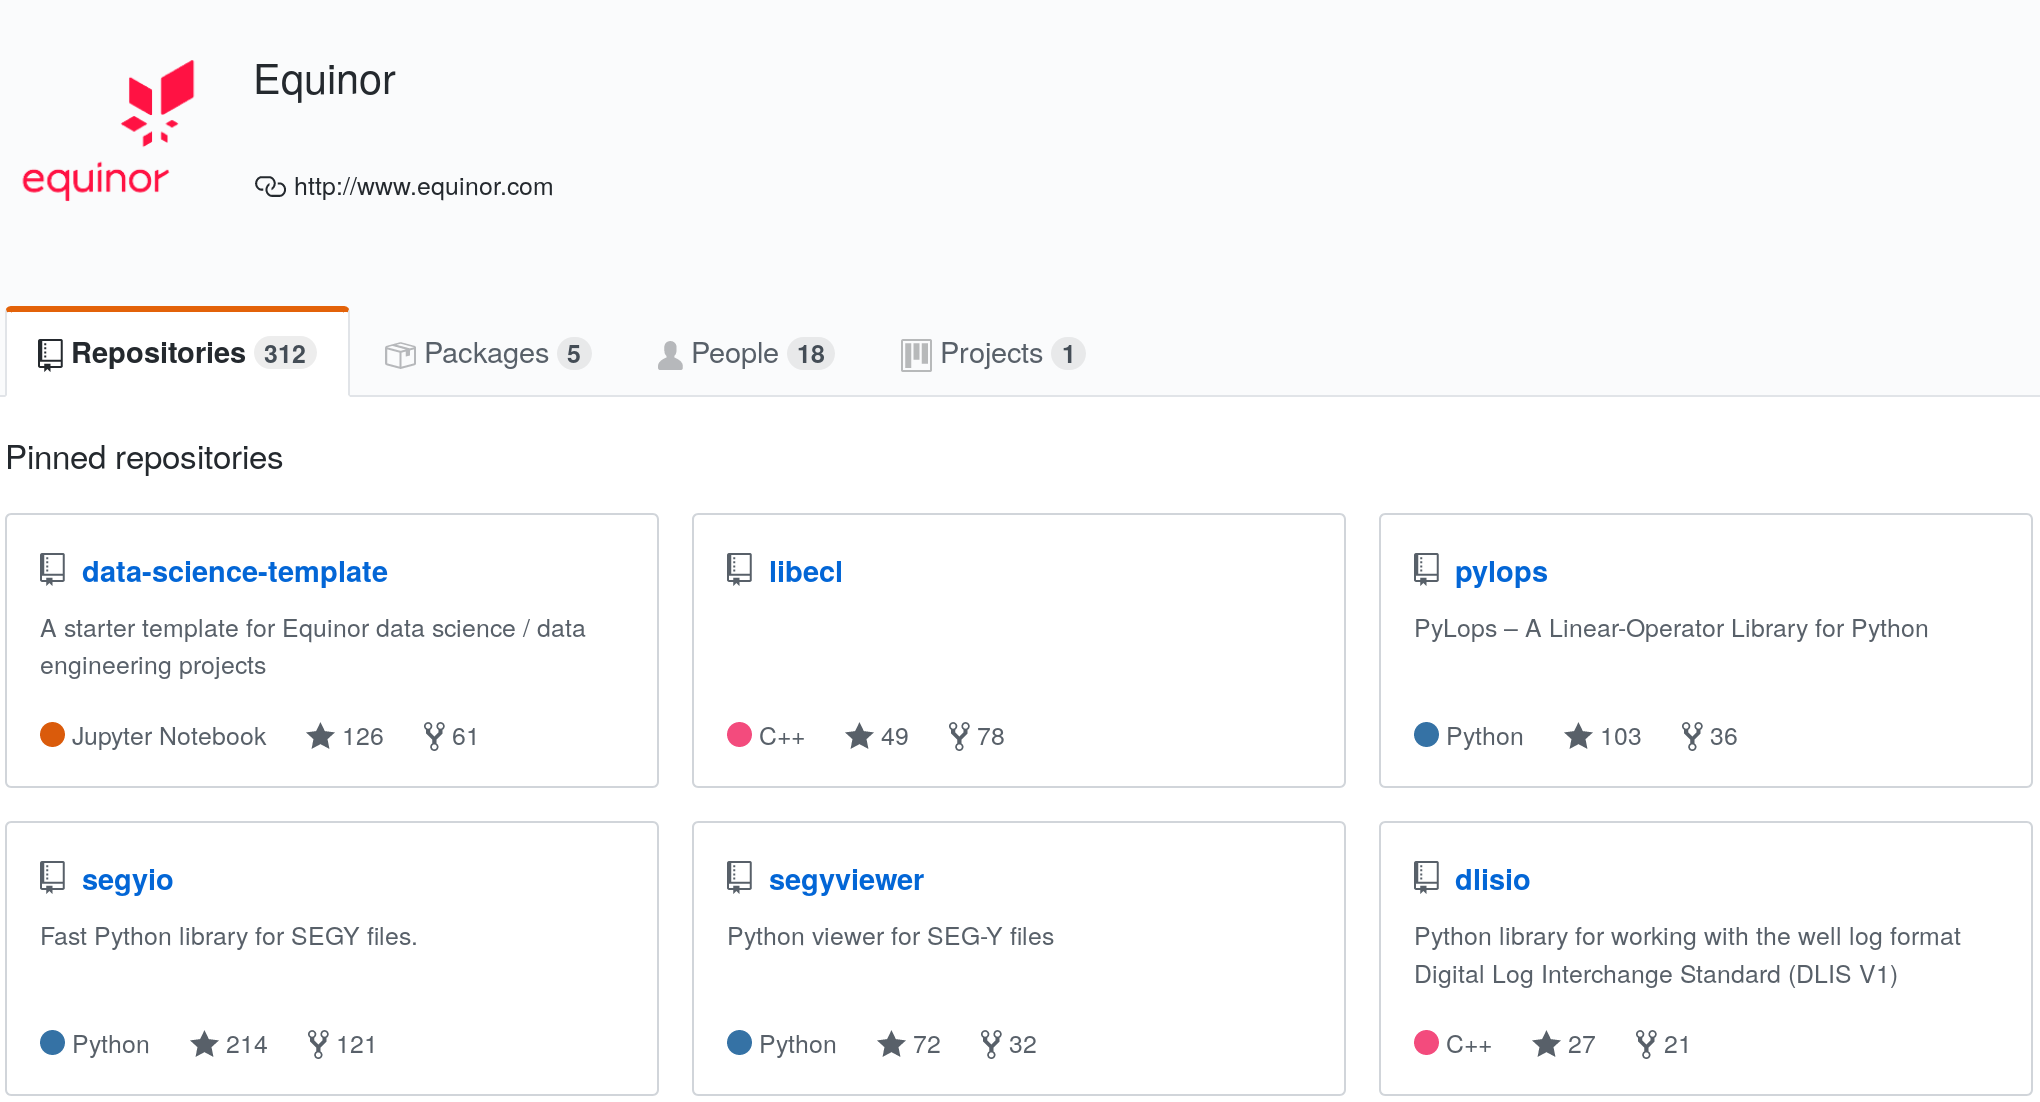
\includegraphics[width=\textwidth, keepaspectratio]{img/equinor-github}
    \begin{center}
        github.com/equinor, May 2020
    \end{center}
\end{frame}

\begin{frame}
    \begin{center}
        \underline{The segyio story}
    \end{center}
\end{frame}

\begin{frame}[fragile]
    \begin{verbatim}
commit 5c05b1bcd9d84da7d383ef03a2f8739a2aaff1f6
Author: Jørgen Kvalsvik <jokva@statoil.com>
Date:   Wed Sep 28 13:53:46 2016 +0200

    Initial commit.
\end{verbatim}
\end{frame}

\begin{frame}
    \begin{center}
        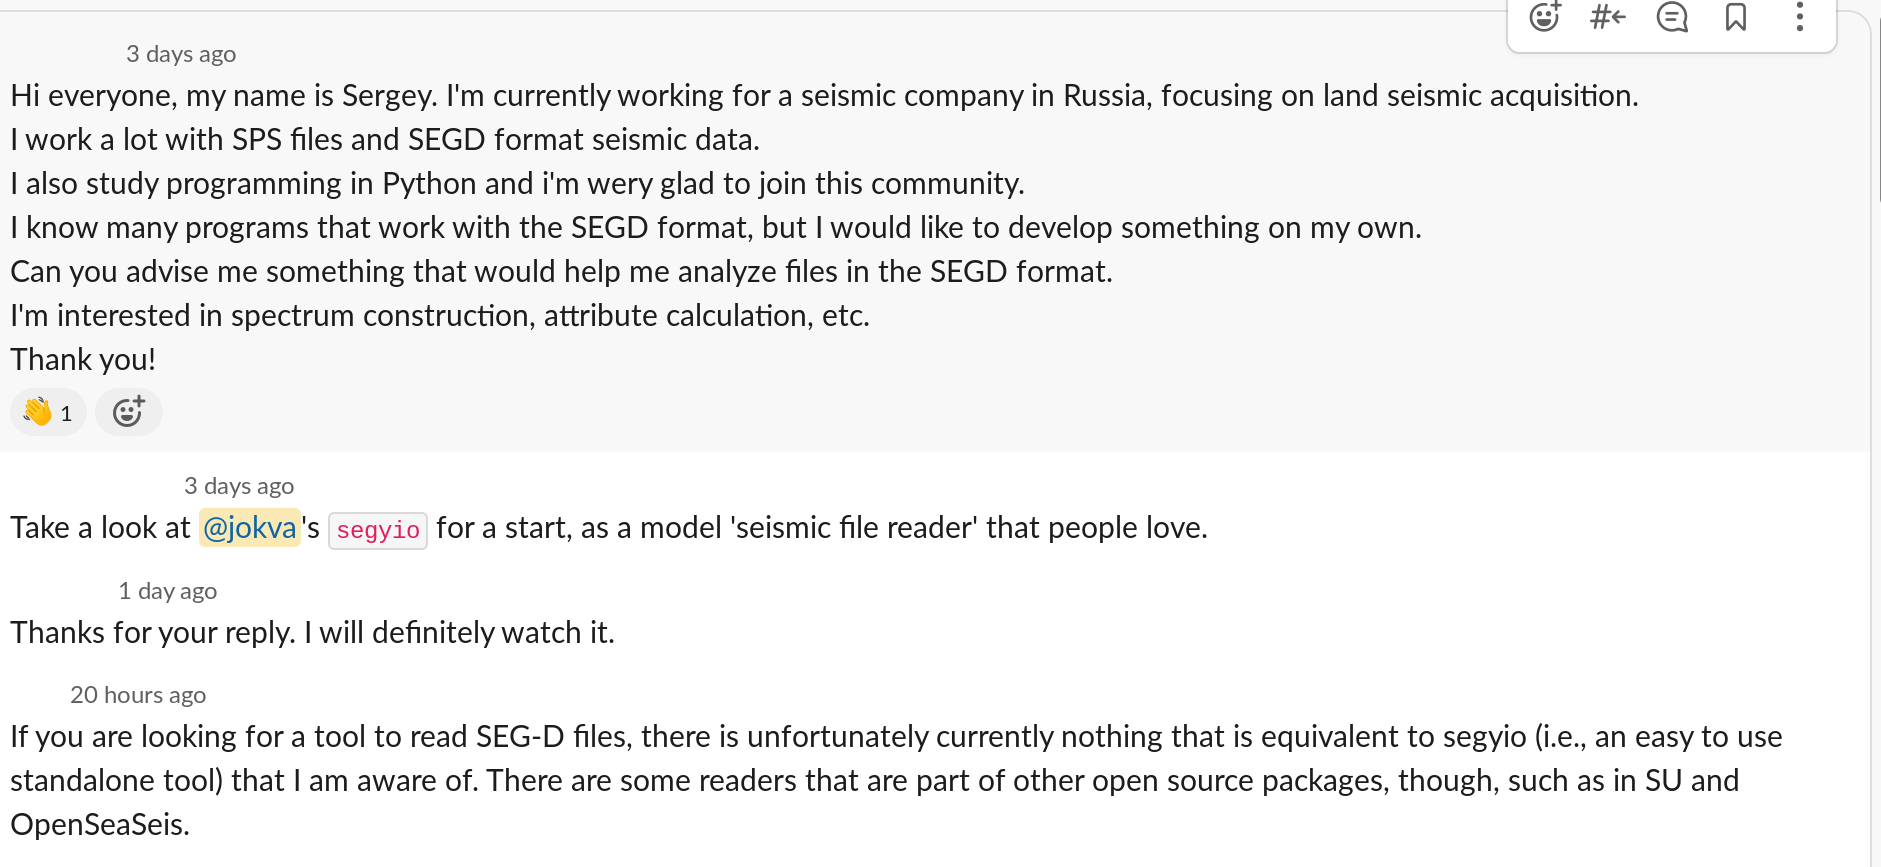
\includegraphics[height=0.5\textheight, keepaspectratio]{img/segyio-praise}
    \end{center}
\end{frame}

\begin{frame}
    \begin{center}
        On development
    \end{center}
\end{frame}

\begin{frame}
    \begin{itemize}
        \item Commisioned in spring 2016, first public release in October
        \item Free software from the start, LGPLv3
        \item Today the de-facto (Python) software for SEG-Y
    \end{itemize}
    First 2-3 months of prototyping was never public
\end{frame}

\begin{frame}
    segyio is built on free software
    \begin{itemize}
        \item gcc and clang, libc
        \item python, numpy
        \item git, vim, cmake
        \item Debian, RHEL
    \end{itemize}
\end{frame}

\begin{frame}
    \begin{center}
        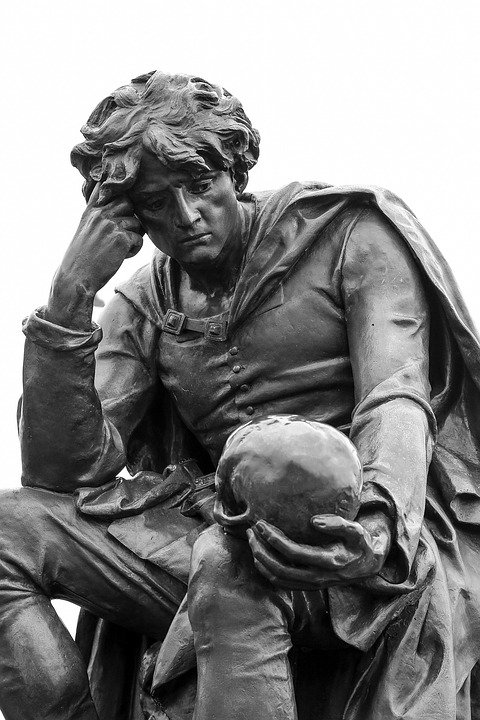
\includegraphics[height=0.8\textheight, keepaspectratio]{img/hamlet-statue}
    \end{center}
\end{frame}

\begin{frame}
    \begin{center}
        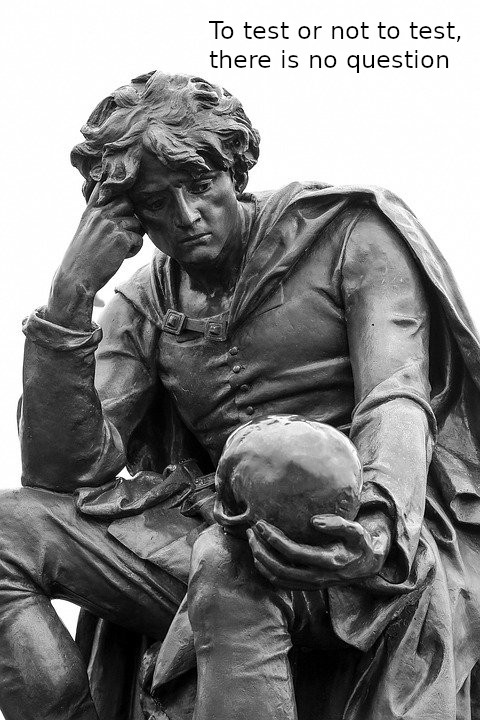
\includegraphics[height=0.8\textheight, keepaspectratio]{img/hamlet-text}
    \end{center}
\end{frame}

\begin{frame}
    \begin{itemize}
        \item Automated test suite from day 1
        \item Single-command build from day 1
        \item Faster and easier to contribute
        \item Faster and easier to maintain
    \end{itemize}

    Automated testing is an essential tool in software development
\end{frame}

\begin{frame}[fragile]
    \begin{verbatim}
commit 2a0e1187abf7fa2fe7aed1118a667462930842a2
Author: Kjell W. Kongsvik <kwko@statoil.com>
Date:   Thu Sep 29 13:44:10 2016 +0200

    travis support
    \end{verbatim}
\end{frame}

\begin{frame}
    Since then tested and used
    \begin{itemize}
        \item Circle CI
        \item Gitlab CI
        \item AppVeyor
        \item Azure Pipelines
        \item Github Pipelines
    \end{itemize}

    Testing a new service is cheap and easy
\end{frame}

\begin{frame}
    Simple building and good tests are useful in non-free projects too

    \begin{itemize}
        \item Easy to bring new developers up to speed
        \item Can quickly set up on new machine
        \item Robust environment less painful, more efficient
        \item Good dev experience gives good software
    \end{itemize}

    Maintaining a good build system is a lot of work
\end{frame}

\begin{frame}[fragile]
    \begin{verbatim}
$ git log --oneline --no-merges | wc -l
806

$ git log --oneline --no-merges --
        CMakeLists.txt
        python/CMakeLists.txt
        python/setup.py
        lib/CMakeLists.txt
    | wc -l
111
    \end{verbatim}
\end{frame}

\begin{frame}
    Open source makes shortcuts more painful
\end{frame}

\begin{frame}
    Amazon API Mandate (2002)

    \begin{displayquote}
        All service interfaces, without exception, must be designed from the
        ground up to be externalizable. That is to say, the team must plan and
        design to be able to expose the interface to developers in the outside
        world. No exceptions.
    \end{displayquote}
\end{frame}

\begin{frame}
    Source code is out there with your name on it
    \begin{itemize}
        \item Be proud and do good work
    \end{itemize}
\end{frame}

\begin{frame}
    Source code is in itself not that valuable
    \begin{itemize}
        \item Behaviour changes when everyone can audit your work
        \item Ability to adapt, modify, and operate is stronger
    \end{itemize}
\end{frame}

\begin{frame}
    Not having to protect source and secrets reduces friction
    \begin{itemize}
        \item Github (public) issue tracker - no jira!
        \item Many services are freely available for open source
        \item Can upload source with no fear, e.g. for static analysis
    \end{itemize}
    Can include actual snippets, no need to paraphrase
\end{frame}

\begin{frame}
    \begin{center}
        On community
    \end{center}
\end{frame}

\begin{frame}
    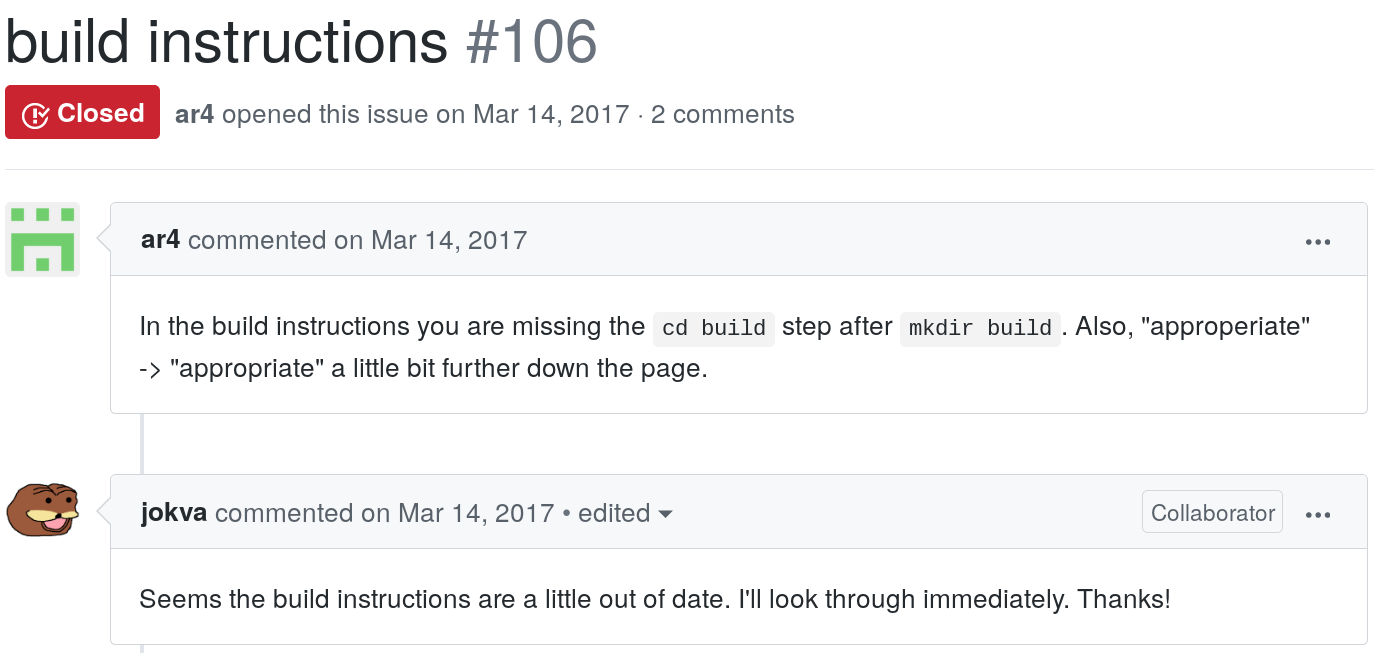
\includegraphics[width=\textwidth, keepaspectratio]{img/segyio-first-issue}
\end{frame}

\begin{frame}
    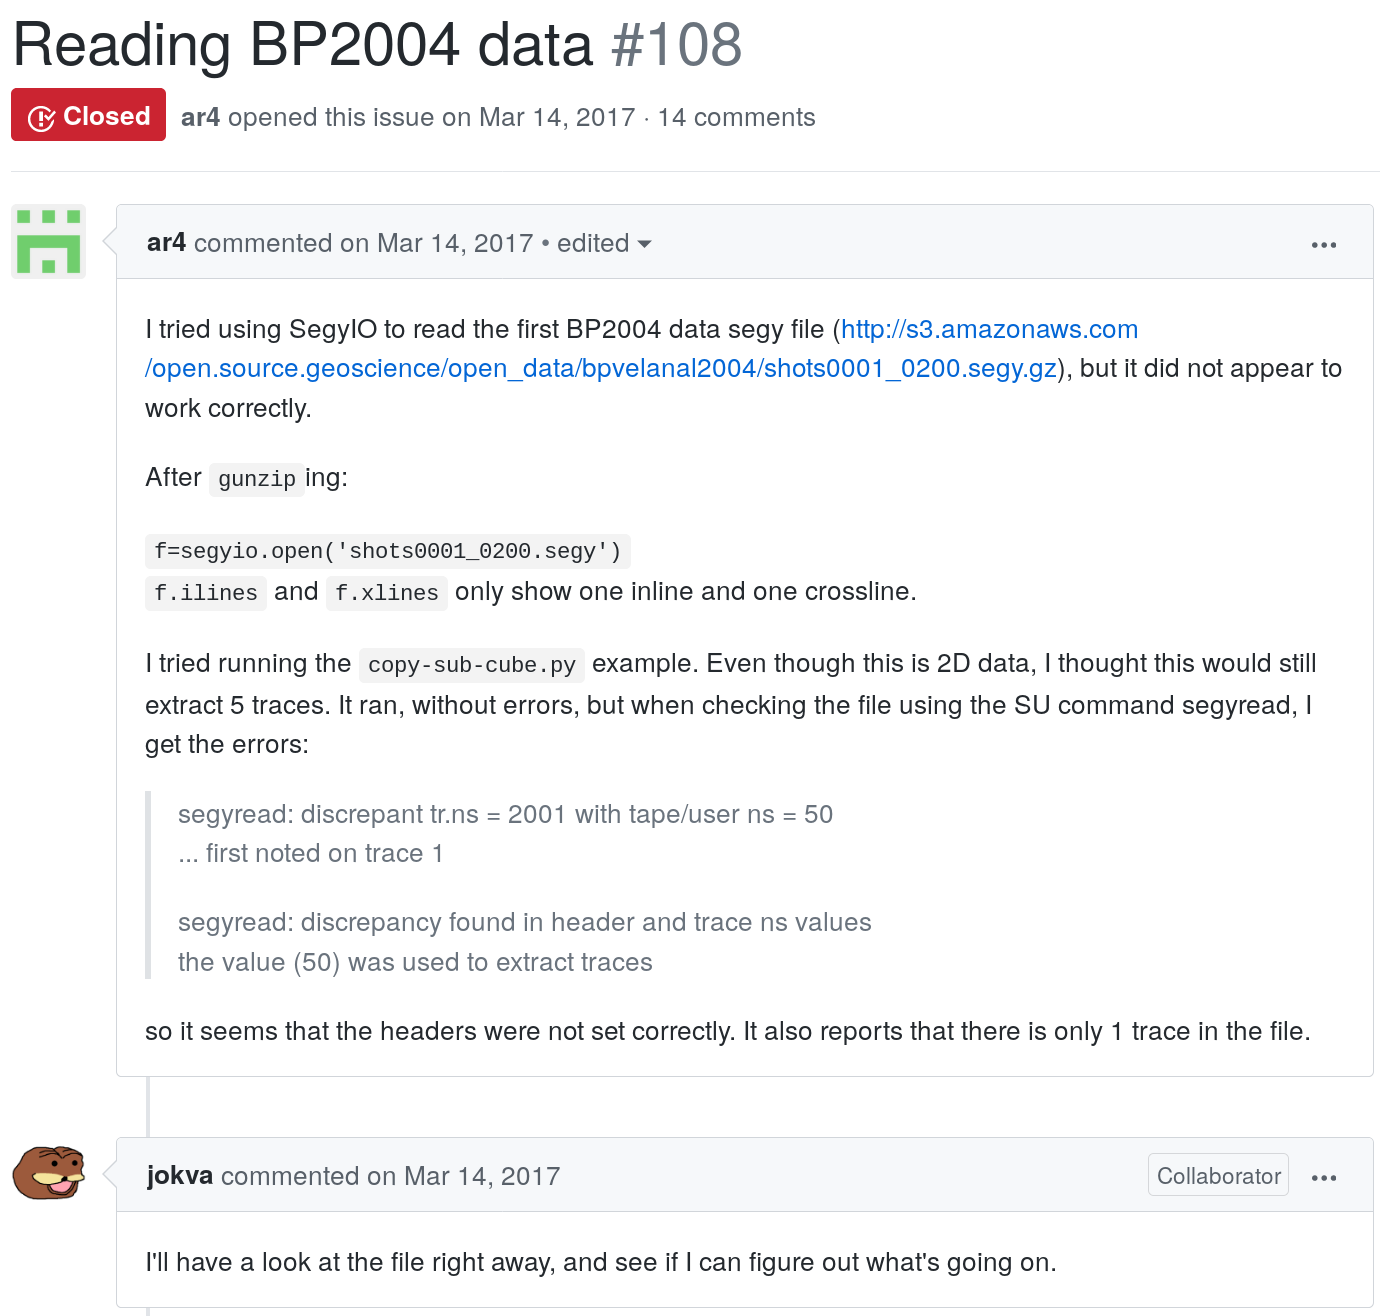
\includegraphics[width=0.8\textwidth, keepaspectratio]{img/segyio-feature-issue}
\end{frame}

\begin{frame}
    segyio added to the wikipedia page \emph{Comparison of free geophysics
    software} 26 April 2017
\end{frame}


\begin{frame}[fragile]
    \begin{Verbatim}[fontsize=\footnotesize]
$ curl -G "https://api.github.com/repos/equinor/segyio/issues"
    | jq ".[].user.login"
    | sort -u
    \end{Verbatim}

    \newcommand{\fade}[1]{\textcolor<2>{gray}{#1}}
    \newcommand{\stay}[1]{\textcolor<2>{black}{#1}}

    \begin{tabular}{l l l}
        \fade{AlbertZhangHIT} & \stay{jokva}          & \fade{sagarnp007}      \\
        \fade{aleran84}       & \fade{ke0m}           & \fade{santaniitr}      \\
        \fade{AlexUser97}     & \fade{kenangogogo}    & \fade{seisgo}          \\
        \fade{ansim58}        & \fade{KirillSimonov}  & \stay{ShikhaMishra9}   \\
        \fade{ar4}            & \fade{kurddt}         & \fade{StefosGeo}       \\
        \fade{doiko}          & \fade{kwinkunks}      & \fade{sumitav}         \\
        \fade{emilsonpl}      & \fade{metazool}       & \fade{superzappie}     \\
        \fade{feel1nwill}     & \fade{nick-falco}     & \stay{sveinung-r}      \\
        \fade{feliperails}    & \fade{nitishkannan23} & \fade{tiulpin}         \\
        \fade{filippo82}      & \fade{pederka}        & \fade{trunlee}         \\
        \fade{GGDRriedel}     & \fade{polarism}       & \fade{valentinmetraux} \\
        \fade{hallgrim}       & \fade{pythonmobile}   & \fade{vkazei}          \\
        \fade{harrymchugh}    & \fade{raplima}        & \fade{wangweiwei104}   \\
        \fade{James-Beckwith} & \fade{rayray313}      & \fade{whimian}         \\
        \fade{JesperDramsch}  & \fade{roelanddeheld}  & \fade{yohanesnuwara}   \\
    \end{tabular}

%https://api.github.com/repos/equinor/segyio/issues?state=all&per_page=100
\end{frame}

\begin{frame}
    Users are a joy, but also a challenge
    \begin{itemize}
        \item In the end, users make software better
        \item A minority of users are entitled and lazy
        \item Most interaction is wonderful and a privilege
    \end{itemize}
    Building community is hard work
\end{frame}

\begin{frame}
    I asked how and why
\end{frame}

\begin{frame}
    \begin{displayquote}
        Needed to load seismic. Obspy and segyio were both options. Tried both.
        Obspy didn't have non-standard headers and was therefore practically
        useless for industry segy files.

        Probably found it through matt/agile or Google
    \end{displayquote}
\end{frame}

\begin{frame}
    \begin{displayquote}
        heard of segyio on swung, choose it because of what looked like the
        most extensive and clear documentation, suggesting (to me) a gentle
        learning curve for a “normal” segy volume
    \end{displayquote}
\end{frame}

\begin{frame}
    \begin{displayquote}
        I've stuck around with segyio because it seemed very easy to interact
        with you the dev as well. Problem or feature missing? Check in if I'm
        doing it wrong.
    \end{displayquote}
\end{frame}

\begin{frame}
    \begin{displayquote}
        ca 4 years ago (?) I was relatively happy and getting increasingly
        comfortable using ObsPy, but I think it was @matt [Agile] who told me
        that segyio was clever and elegant in the way that it handled headers
        particularly in shaping traces into cubes. It felt magical using that
        with a context manager.
    \end{displayquote}
\end{frame}


\begin{frame}
    \begin{displayquote}
        I'm a few days late to this topic, but I'll share my experience with segyio. I
        found the software via Google search the same week I started learning
        Python as a first language (well before I knew about Swung). I needed
        to tackle a specific problem that my available commercial software
        couldn't handle. I also looked at ObsPy, but segyio seemed more
        fit-for-purpose with a gentler learning curve. Speaking to community,
        when I asked a simple newbie question on GitHub during that first week
        of coding (pasting my code without triple backticks, even!), I was
        given plenty of helpful debugging advice that let me accomplish that
        near-term goal. That welcoming attitude is how you build a community
    \end{displayquote}
\end{frame}

\begin{frame}
    \begin{displayquote}
        ... use version 1.3 because other versions have problems
    \end{displayquote}
\end{frame}

\begin{frame}
    User interaction all the time
    \begin{itemize}
        \item Issue tracker
        \item Software Underground
        \item Email
        \item Hackathons and conferences (NDC!)
        \item Subsurface Copenhagen 2018, Transform 2019
        \item EAGE London 2019
    \end{itemize}

    Taking care of users is a part of maintaining software
\end{frame}

\begin{frame}
    The community gives back!

    \begin{itemize}
        \item Feedback and testing
        \item New use cases
        \item Feature suggestions
        \item Users help users
    \end{itemize}
\end{frame}

\begin{frame}
    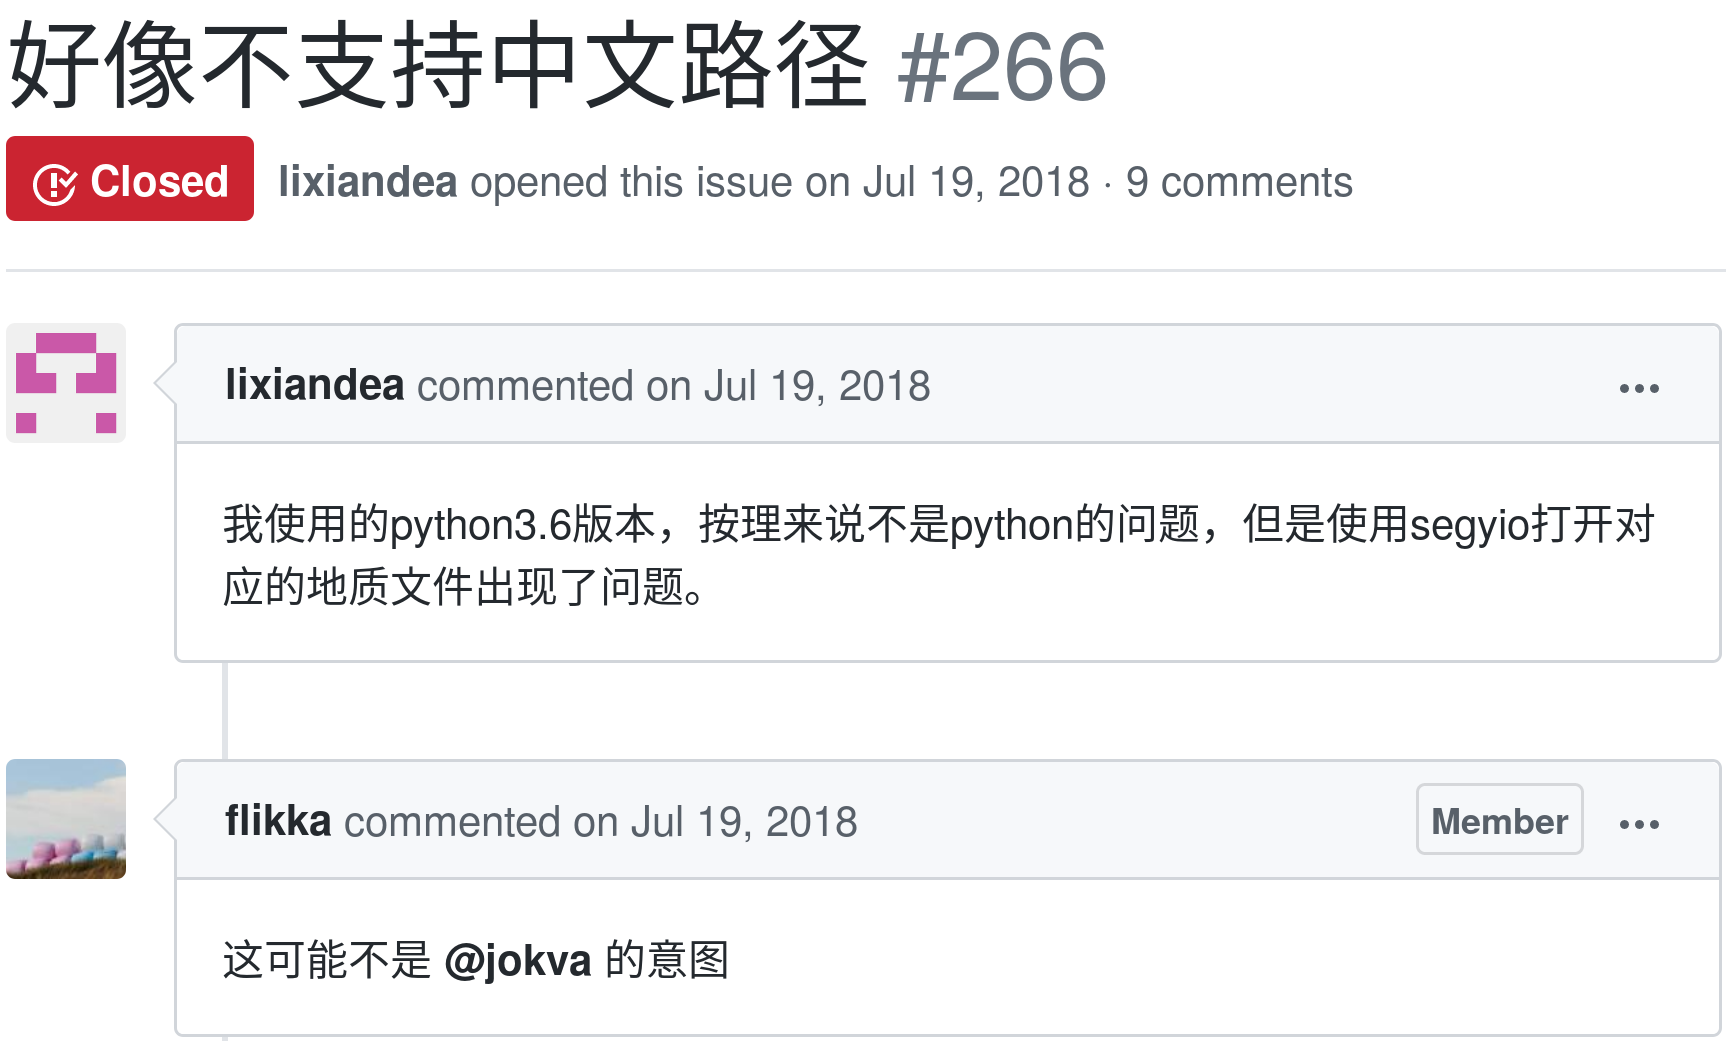
\includegraphics[width=\textwidth, keepaspectratio]{img/segyio-sino}
\end{frame}

\begin{frame}
    Fairly few code contributions -- 195/20k live LOC, including docs
\end{frame}

\begin{frame}
    \textbf{Open-Source, not Open-Contribution}
    \begin{displayquote}
        SQLite is open-source, meaning that you can make as many copies of it as you
        want and do whatever you want with those copies, without limitation. But SQLite
        is not open-contribution.
    \end{displayquote}

    https://www.sqlite.org/copyright.html
\end{frame}

\begin{frame}
    \begin{center}
        On packaging, distribution, and documentation
    \end{center}
\end{frame}

\begin{frame}
    \begin{itemize}
        \item Source tarball
        \item Python wheels and pip install
        \item Debian package
        \item Conda package
    \end{itemize}
    Most Equinor users use the pip package
\end{frame}

\begin{frame}
    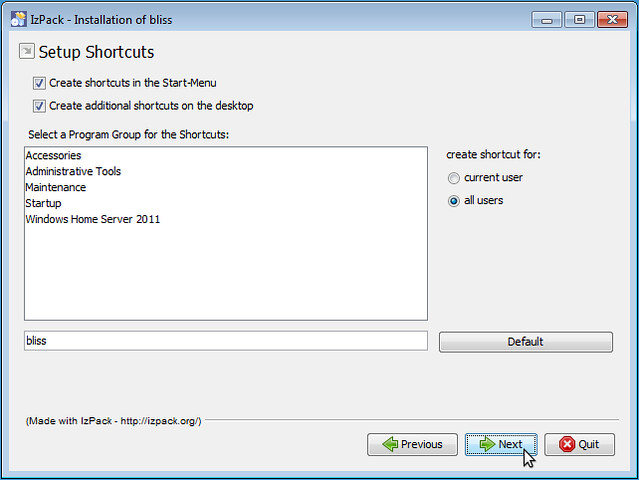
\includegraphics[width=\textwidth, keepaspectratio]{img/installer}
\end{frame}

\begin{frame}
    Can no longer tie to company internals

    \begin{itemize}
        \item Enterprise doc systems are awful
        \item Keeps docs honest
        \item Community!
    \end{itemize}
\end{frame}

\begin{frame}
    \begin{center}
        On politics and money
    \end{center}
\end{frame}

\begin{frame}
    Open sourcing will not solve issues in organization
    \begin{itemize}
        \item Underfunding
        \item Mismanagement, lack of direction
        \item Lack of understanding
    \end{itemize}
    But it \emph{will} empower your users and soften the blow
\end{frame}

\begin{frame}
    \begin{displayquote}
        There is probably never a once and for all for anything but more a good
        enough for now, and then let the open (source) market make improvements
        to the code such that finally for all is achieved in the future.
    \end{displayquote}
\end{frame}

\begin{frame}
    \begin{center}
        There is no free lunch
    \end{center}
    \begin{figure}
        
\includegraphics[width=\textwidth, keepaspectratio]{img/cake}
    \end{figure}
\end{frame}

\begin{frame}
    \begin{center}
        Postlude
    \end{center}
\end{frame}

\begin{frame}
    Retrospective on segyio
\end{frame}

\begin{frame}
    Would I do it again?
\end{frame}

\begin{frame}{Thank you}
    
\includegraphics[width = \textwidth]{img/porcorosso}
\end{frame}

\end{document}
